\section{Results}
\label{Results}
%
Of the 10 green categories, four categories are exemplified which are related to the robot’s Appearance (udseende), Trust (tillid), Behaviour (væremåde), and Approach (henvendelse). Based on these categories a variable can be elicited according to the criterion of a) being an influencing variable and b) the possibility of formulating the variable as a scale question. The field study was conducted on Danish speaking test subjects, and the variables are listed in both English and Danish. For each of the four categories the following statements are derived from the affinity diagram and will later serve as a basis for the potential scale. \textit{R} is short for robot.\\
%
\begin{itemize}
\item Appearance
\begin{enumerate}
  \item I think R's height is... (Jeg synes at R's højde er...)
  \item I think R is elegant... (Jeg synes R er elegant...)
  \item I think R looks human... (Jeg synes R ser menneskelig ud...)
  \item I like R's appearance... (Jeg kan godt lide R's udseende...)\\
\end{enumerate}
\item Trust 
\begin{enumerate}
  \item I feel safe around R (Jeg føler mig tryg ved R)
  \item I expect that R leads me to the chosen place (Jeg regner med at R følger mig hen til det sted jeg har valgt)
  \item R startled me (R gjorde mig forskrækket)\\
\end{enumerate}
\item Behaviour
\begin{enumerate}
  \item I think R's movements are... (Jeg synes R's bevægelser er...)
  \item I think R's speed is... (Jeg synes at R's hastighed er...)
  \item I think R is annoying... (Jeg synes R er irriterende...)
  \item I think R is alive... (Jeg synes R er levende...)
  \item I think R is intrusive... (Jeg synes R er anmassende...)\\
\end{enumerate}
\item Approach 
\begin{enumerate}
  \item I think R is welcoming (Jeg synes R er imødekommende)
  \item I think that R came too close to me (Jeg synes R kom for tæt på)
  \item I think that R was obstructive... (Jeg synes R stod i vejen)
  \item I was surprised by R's approach (Jeg blev overrasket over R's henvendelse)
  \item I thought that R was intimidating (Jeg synes R er intimiderende)\\
\end{enumerate}
\end{itemize}
%
When comparing the variables for HRI found in this study with variables for HRI from previous conducted studies on social robots \cite{PDF:ExploringInfluencingVariable}, \cite{PDF:SharingALifeHarvey}, \cite{PDF:InTheCompanyofRobots}, \cite{PDF:CloseButNotStuck}, \cite{PDF:TheImpactOfTraveler}, \cite{PDF:HumanRobotEmodiedInteraction}, \cite{PDF:RecommendationEffects}, variables such as distance, anthropomorphism, height, speed, movement, trust, and usefulness reoccur. New variables were found compared with previous mentioned studies. Under appearance such a variable is elegance. There was only found one new variable under trust which was if the robot startle you. According to behaviour the new variables found are how annoying and intrusive the robot was, and how calm or wild the movements of the robot were. Focusing on approach the new variables are how welcoming, obstructive, surprising, and intimidating the robot is perceived. In the following tables each individual scale question, noted with \textit{SQ}, is listed alongside the labels on the specific scale. If the scale does not contain a mid point it will be noted with \textit{-}, if it contains an unlabelled mid point it will be noted with \textit{No label}, whereas if the mid point is labelled the specific label is noted. 
%
\begin{table}[H]
	\centering
\caption{Scale labels for the robot's appearance}
	\label{tab:AppearanceScale} 
	\begin{tabular}{l|c|c|c}
		SQ     & Left label & Mid point & Right label \\\hline
		1   & \makecell{Too low \\(for lav)}  & \makecell{Appropriate \\(fin)} & \makecell{Too high \\(for høj)}        \\\hline
		2   & \makecell{Not at all elegant \\(slet ikke elegant)} & - & \makecell{Extremely elegant \\(ekstremt elegant)}         \\\hline
		3   & \makecell{Not at all human \\(slet ikke menneskelig)} & - & \makecell{Extremely human \\(ekstremt menneskelig)}         \\\hline
	 	4   & \makecell{Completely disagree \\(helt uenig)} & - & \makecell{Completely agree \\(helt enig)}         \\\hline
		5   & \makecell{Not at all startled \\(slet ikke forskrækket)} & -  & \makecell{Extremely startled \\(ekstremt forskrækket)}           
	\end{tabular}        
\end{table}
\noindent
%
%
\begin{table}[H]
	\centering
\caption{Scale labels regarding trust}
	\label{tab:TrustScale} 
	\begin{tabular}{l|c|c|c}
		SQ  & Left label & Mid point & Right label \\\hline
		1   & \makecell{Extremely unsafe\\ (ekstremt utryg)} & No label & \makecell{Extremely safe \\(ekstremt tryg)}          \\\hline
		2   & \makecell{Completely disagree \\(helt uenig)} & Neutral &\makecell{Completely agree \\(helt enig)} 
	\end{tabular}        
\end{table}
\noindent
%
%
\begin{table}[H]
	\centering
\caption{Scale labels for the robot's behaviour}
	\label{tab:BehaviorScale} 
	\begin{tabular}{l|c|c|c}
		SQ     & Left label & Mid point & Right label \\\hline
		1   & \makecell{Too calm \\(for rolige)} & No label & \makecell{Too wild \\(for vilde)}           \\\hline
		2   & \makecell{Too slow \\(for langsom)} & \makecell{Appropriate \\(fin)} & \makecell{Too fast \\(for hurtig)}   \\\hline
		3   & \makecell{Not at all annoying \\(slet ikke irriterende)} & - & \makecell{Extremely annoying \\(ekstremt irriterende)}          \\\hline
	 	4   & \makecell{Not at all alive \\(slet ikke levende)} & - & \makecell{Extremely alive \\(ekstremt levende)}         \\\hline
		5   & \makecell{Not at all intrusive \\(slet ikke anmassende)} & - & \makecell{Extremely intrusive \\(ekstremt anmassende)}             
	\end{tabular}
\end{table}
\noindent
%
%
\begin{table}[H]
	\centering
\caption{Scale labels for the robot's approach}
	\label{tab:ApproachScale} 
	\begin{tabular}{l|c|c|c}
		SQ     & Left label & Mid point & Right label \\\hline
		1   & \makecell{Very unwelcoming \\(meget afvisende)} & No label & \makecell{Very welcoming \\(meget imødekommende)}          \\\hline
		2   & \makecell{Too far \\(for langt væk)} & \makecell{Appropriate \\(tilpas)} & \makecell{Too close \\(for tæt på)}          \\\hline
		3   & \makecell{Not at all obstructive \\(slet ikke i vejen)}& -  & \makecell{Extremely obstructive \\(ekstremt i vejen)}  \\\hline
	 	4   & \makecell{Not at all surprised \\(slet ikke overrasket)} &  -  & \makecell{Extremely surprised \\(ekstremt overrasket)}       \\\hline
		5   & \makecell{Not at all intimidating \\(slet ikke intimiderende)} & - & \makecell{Extremely intimidating \\(ekstremt intimiderende)}           
	\end{tabular}
\end{table}
\noindent
%
The scale questions are presented on a \textit{Visual Analoge Scale} (VAS) with open anchor points, with or without mid point markers, and are either bi- or unipolar. If the scale is bipolar a mid point will be marked either with or without a label. Each scale consists of its own specific labels which are listed in \autoref{tab:AppearanceScale} for robot appearance, \autoref{tab:TrustScale} for robot trust,\autoref{tab:BehaviorScale} for robot behaviour, and \autoref{tab:ApproachScale} for robot approach. At the time of writing, the scales have not finally been developed but are expected to appear as shown on \autoref{fig:Height} for a bipolar scale with labelled mid point. 
%
\begin{figure}[H]
\centering
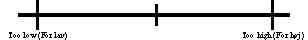
\includegraphics[width = 0.49\textwidth]{Figure/HeightHoejde} 
\caption{Example of a bipolar scale with a labeled mid point relevant for the scale question: \textit{I think R's height is...}}
\label{fig:Height}
\end{figure}
\noindent
% 
A bipolar scale without a label is expected to appear as shown on \autoref{fig:Calm}.  
%
\begin{figure}[H]
\centering
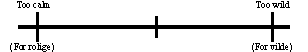
\includegraphics[width = 0.49\textwidth]{Figure/CalmWild} 
\caption{Example of a bipolar scale without a labeled mid point relevant for the scale question: \textit{I think R's movements are...}}
\label{fig:Calm}
\end{figure}
\noindent
%
An example of an unipolar scale as it is expected to appear is shown on \autoref{fig:HumanMenneskelig}.
%
\begin{figure}[H]
\centering
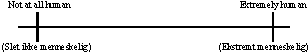
\includegraphics[width = 0.49\textwidth]{Figure/HumanMenneskelig} 
\caption{Example of an unipolar scale relevant for the scale question: \textit{I think R looks human}.}
\label{fig:HumanMenneskelig}
\end{figure}
\noindent
%

